% Options for packages loaded elsewhere
\PassOptionsToPackage{unicode}{hyperref}
\PassOptionsToPackage{hyphens}{url}
\documentclass[
  11pt,
]{article}
\usepackage{xcolor}
\usepackage[left=3cm,right=3cm,top=2.5cm,bottom=2.5cm]{geometry}
\usepackage{amsmath,amssymb}
\setcounter{secnumdepth}{5}
\usepackage{iftex}
\ifPDFTeX
  \usepackage[T1]{fontenc}
  \usepackage[utf8]{inputenc}
  \usepackage{textcomp} % provide euro and other symbols
\else % if luatex or xetex
  \usepackage{unicode-math} % this also loads fontspec
  \defaultfontfeatures{Scale=MatchLowercase}
  \defaultfontfeatures[\rmfamily]{Ligatures=TeX,Scale=1}
\fi
\usepackage{lmodern}
\ifPDFTeX\else
  % xetex/luatex font selection
\fi
% Use upquote if available, for straight quotes in verbatim environments
\IfFileExists{upquote.sty}{\usepackage{upquote}}{}
\IfFileExists{microtype.sty}{% use microtype if available
  \usepackage[]{microtype}
  \UseMicrotypeSet[protrusion]{basicmath} % disable protrusion for tt fonts
}{}
\usepackage{setspace}
\makeatletter
\@ifundefined{KOMAClassName}{% if non-KOMA class
  \IfFileExists{parskip.sty}{%
    \usepackage{parskip}
  }{% else
    \setlength{\parindent}{0pt}
    \setlength{\parskip}{6pt plus 2pt minus 1pt}}
}{% if KOMA class
  \KOMAoptions{parskip=half}}
\makeatother
\usepackage{longtable,booktabs,array}
\usepackage{caption}
\captionsetup[table]{skip=6pt}
\newcounter{none} % for unnumbered tables
\usepackage{calc} % for calculating minipage widths
% Correct order of tables after \paragraph or \subparagraph
\usepackage{etoolbox}
\makeatletter
\patchcmd\longtable{\par}{\if@noskipsec\mbox{}\fi\par}{}{}
\makeatother
% Allow footnotes in longtable head/foot
\IfFileExists{footnotehyper.sty}{\usepackage{footnotehyper}}{\usepackage{footnote}}
\makesavenoteenv{longtable}
\usepackage{graphicx}
\makeatletter
\newsavebox\pandoc@box
\newcommand*\pandocbounded[1]{% scales image to fit in text height/width
  \sbox\pandoc@box{#1}%
  \Gscale@div\@tempa{\textheight}{\dimexpr\ht\pandoc@box+\dp\pandoc@box\relax}%
  \Gscale@div\@tempb{\linewidth}{\wd\pandoc@box}%
  \ifdim\@tempb\p@<\@tempa\p@\let\@tempa\@tempb\fi% select the smaller of both
  \ifdim\@tempa\p@<\p@\scalebox{\@tempa}{\usebox\pandoc@box}%
  \else\usebox{\pandoc@box}%
  \fi%
}
% Set default figure placement to htbp
\def\fps@figure{htbp}
\makeatother
% definitions for citeproc citations
\NewDocumentCommand\citeproctext{}{}
\NewDocumentCommand\citeproc{mm}{%
  \begingroup\def\citeproctext{#2}\cite{#1}\endgroup}
\makeatletter
 % allow citations to break across lines
 \let\@cite@ofmt\@firstofone
 % avoid brackets around text for \cite:
 \def\@biblabel#1{}
 \def\@cite#1#2{{#1\if@tempswa , #2\fi}}
\makeatother
\newlength{\cslhangindent}
\setlength{\cslhangindent}{1.5em}
\newlength{\csllabelwidth}
\setlength{\csllabelwidth}{3em}
\newenvironment{CSLReferences}[2] % #1 hanging-indent, #2 entry-spacing
 {\begin{list}{}{%
  \setlength{\itemindent}{0pt}
  \setlength{\leftmargin}{0pt}
  \setlength{\parsep}{0pt}
  % turn on hanging indent if param 1 is 1
  \ifodd #1
   \setlength{\leftmargin}{\cslhangindent}
   \setlength{\itemindent}{-1\cslhangindent}
  \fi
  % set entry spacing
  \setlength{\itemsep}{#2\baselineskip}}}
 {\end{list}}
\usepackage{calc}
\newcommand{\CSLBlock}[1]{\hfill\break\parbox[t]{\linewidth}{\strut\ignorespaces#1\strut}}
\newcommand{\CSLLeftMargin}[1]{\parbox[t]{\csllabelwidth}{\strut#1\strut}}
\newcommand{\CSLRightInline}[1]{\parbox[t]{\linewidth - \csllabelwidth}{\strut#1\strut}}
\newcommand{\CSLIndent}[1]{\hspace{\cslhangindent}#1}
\setlength{\emergencystretch}{3em} % prevent overfull lines
\providecommand{\tightlist}{%
  \setlength{\itemsep}{0pt}\setlength{\parskip}{0pt}}
% Statistics in Medicine submission preamble.
% Shared across analysis/report/<paper>/report.Rmd files via
%   includes:
%     in_header: ../sim-preamble.tex
% in the YAML output block.
%
% The page footer (source path, render time, version) is no
% longer set here. It is supplied at render time by the vendored
% tools/stamp-render.R, which injects tools/stamp.tex.

% Continuous line numbering for editorial review. The 'mathlines'
% option extends numbering through display-math environments
% (equation, align, ...), which SIM editorial workflows expect.
\usepackage[mathlines]{lineno}
\linenumbers
\usepackage{amsmath}

% Spacing: linestretch is set in YAML (1.5 line spacing).
\usepackage{setspace}
%% tools/stamp.tex
%% Provenance footer for PDFs rendered from this project.
%% Vendored by zzcollab; this file is not project-specific. The
%% footer prints the source document and the time of rendering.
%% The git version is defined here too, and so is available to a
%% project that wants it on the page, but it is left off the
%% default footer: it already names the staged copy in share/ and
%% appears in its manifest row. All values are supplied at render
%% time by tools/stamp-render.R, which writes a small generated
%% file that redefines the macros below. The \providecommand
%% defaults keep a bare LaTeX compile working when the document is
%% built without the wrapper.
\usepackage{fancyhdr}
\usepackage{xcolor}
\providecommand{\stampsource}{\detokenize{(source not recorded)}}
\providecommand{\stamptime}{(time not recorded)}
\providecommand{\stampversion}{\detokenize{(version not recorded)}}
\setlength{\footskip}{40pt}
\newcommand{\stampfootcontent}{%
  \footnotesize\color{gray}%
  \parbox[b]{\textwidth}{%
    \stamptime\hfill\thepage\\[2pt]%
    \ttfamily\raggedright\stampsource}}
\pagestyle{fancy}
\fancyhf{}
\fancyfoot[C]{\stampfootcontent}
\renewcommand{\headrulewidth}{0pt}
\renewcommand{\footrulewidth}{0.4pt}
%% The title page uses the `plain` page style; redefine it so the
%% stamp appears there too.
\fancypagestyle{plain}{%
  \fancyhf{}%
  \fancyfoot[C]{\stampfootcontent}%
  \renewcommand{\headrulewidth}{0pt}%
  \renewcommand{\footrulewidth}{0.4pt}}
\renewcommand{\stampsource}{\textasciitilde{}/\allowbreak{}prj/\allowbreak{}res/\allowbreak{}36-pmsimstats-ng/\allowbreak{}pmsimstats-ng/\allowbreak{}analysis/\allowbreak{}report/\allowbreak{}02-carryover-sensitivity/\allowbreak{}supplement.Rmd}
\renewcommand{\stamptime}{2026-08-19 11:36 PDT}
\renewcommand{\stampversion}{\detokenize{3f8423f-wip}}
\usepackage{amsmath}
\usepackage{amssymb}
\usepackage{booktabs}
\usepackage{longtable}
\usepackage{float}
\usepackage[mathlines]{lineno}
\linenumbers
\usepackage{booktabs}
\usepackage{longtable}
\usepackage{array}
\usepackage{multirow}
\usepackage{wrapfig}
\usepackage{float}
\usepackage{colortbl}
\usepackage{pdflscape}
\usepackage{tabu}
\usepackage{threeparttable}
\usepackage{threeparttablex}
\usepackage[normalem]{ulem}
\usepackage{makecell}
\usepackage{xcolor}
\usepackage{bookmark}
\IfFileExists{xurl.sty}{\usepackage{xurl}}{} % add URL line breaks if available
\urlstyle{same}
% fallback for those not using the hyperref driver hyperxmp:
\makeatletter
\@ifundefined{xmpquote}{\newcommand{\xmpquote}[1]{#1}}{}
\makeatother
\hypersetup{
  pdftitle={Supplement: Carryover representation and inference for biomarker-treatment interaction tests in aggregated N-of-1 trials under covariance moderation},
  pdfauthor={pmsimstats team},
  hidelinks,
  pdfcreator={LaTeX via pandoc}}

\title{Supplement: Carryover representation and inference for biomarker-treatment interaction tests in aggregated N-of-1 trials under covariance moderation}
\author{pmsimstats team}
\date{August 19, 2026}

\begin{document}
\maketitle

{
\setcounter{tocdepth}{2}
\tableofcontents
}
\setstretch{1.1}
\emph{This document is a companion to the manuscript ``Carryover
representation and inference for biomarker-treatment interaction
tests in aggregated N-of-1 trials under covariance moderation: a
factorial simulation comparison of nine analysis specifications''
(pmsimstats team). The main manuscript was
kept to a working length by moving six of its eleven Tier 2
sensitivity blocks here in full (S1, S4, S10, S11) or in part (S2,
S8; the main text keeps each block's headline finding and a
one-paragraph summary, with the full cell-by-cell detail below). A
final section (S12) is exploratory material outside the main
manuscript's stated scope: an Architecture A (mean moderation)
counterpart to the main manuscript's Figures 1-3, included here for
comparison only. Block, specification, and G-code notation match the
main manuscript exactly; this supplement does not stand on its own
and should be read alongside it.}

\bigskip\noindent

\rule{\textwidth}{0.4pt}\bigskip

\section{S1: within-factor autocorrelation}\label{s1-within-factor-autocorrelation}

The main text (Section 3.6) summarizes this block's finding: the
Exposure-weighted advantage is preserved at every autocorrelation
level examined. Full detail follows.

\begin{figure}
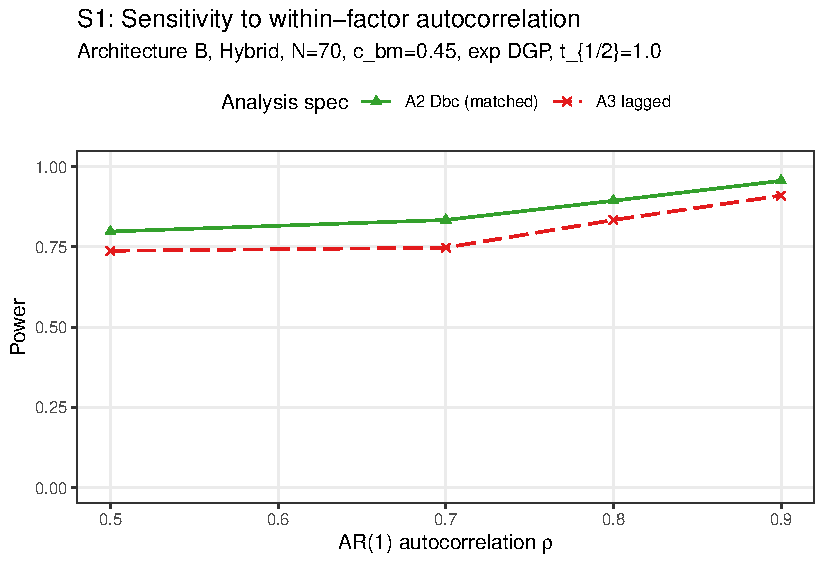
\includegraphics[width=0.6\linewidth]{../../figures/02xs-sens-S1} \caption{Power by analysis specification across AR(1) autocorrelation $\rho \in \{0.5, 0.7, 0.8, 0.9\}$.}\label{fig:fig-sens-s1}
\end{figure}

\begin{figure}
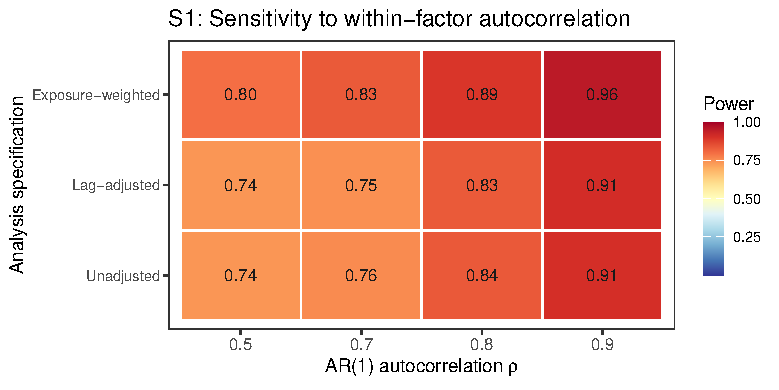
\includegraphics[width=0.7\linewidth]{../../figures/02xs-heatmap-sens-S1} \caption{Block S1: power by AR(1) autocorrelation and analysis specification, same data as the line plot above.}\label{fig:fig-heatmap-sens-s1}
\end{figure}

\begin{figure}
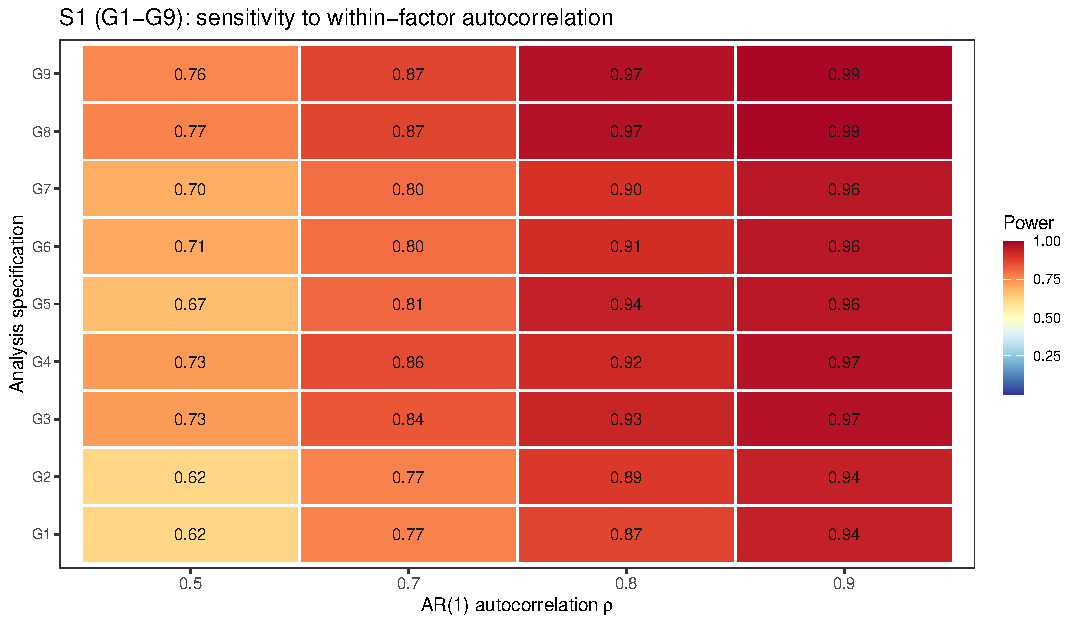
\includegraphics[width=0.8\linewidth]{../../figures/02xs-heatmap-sens-S1-g9} \caption{Block S1 extended to all nine G1-G9 specifications (preliminary $n_{sim} = 100$).}\label{fig:fig-heatmap-sens-s1-g9}
\end{figure}

All three specifications gain power monotonically with \(\rho\), from
\(0.798 \pm 0.018\) (Exposure-weighted) and \(0.738 \pm 0.020\) (the
other two, identical to three decimals) at \(\rho = 0.5\), to
\(0.956 \pm 0.009\) against \(0.906\) to \(0.910\) at \(\rho = 0.9\). The
Exposure-weighted advantage, roughly 0.05 to 0.08 in absolute power,
is preserved at every autocorrelation level examined, suggesting
autocorrelation strength and specification choice act additively
rather than interacting. Lag-adjusted tracks Unadjusted throughout,
never differing by more than 0.008.

\section{S2: analyst-truth half-life mismatch, full detail}\label{s2-analyst-truth-half-life-mismatch-full-detail}

The main text (Section 3.6) reports this block's practical
conclusion: an approximate half-life is adequate, with under-assuming
safer than over-assuming. Full cell-by-cell detail follows.

\begin{figure}
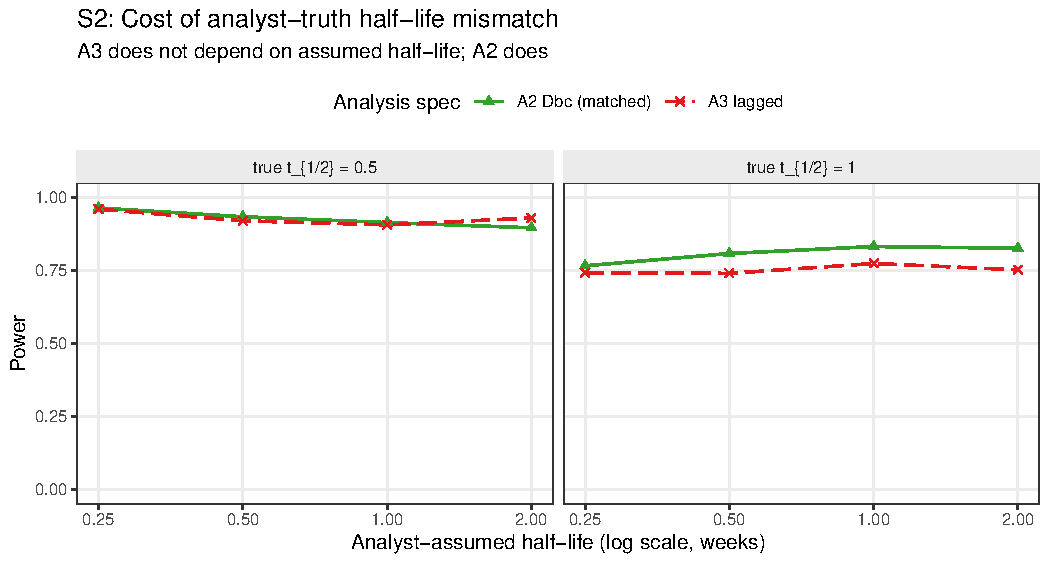
\includegraphics[width=0.8\linewidth]{../../figures/02xs-sens-S2} \caption{Power as the analyst's assumed half-life departs from the true DGP half-life. Only Exposure-weighted consumes the assumed half-life. Unadjusted and Lag-adjusted are invariant to it by construction and appear as flat reference lines.}\label{fig:fig-sens-s2}
\end{figure}

\begin{figure}
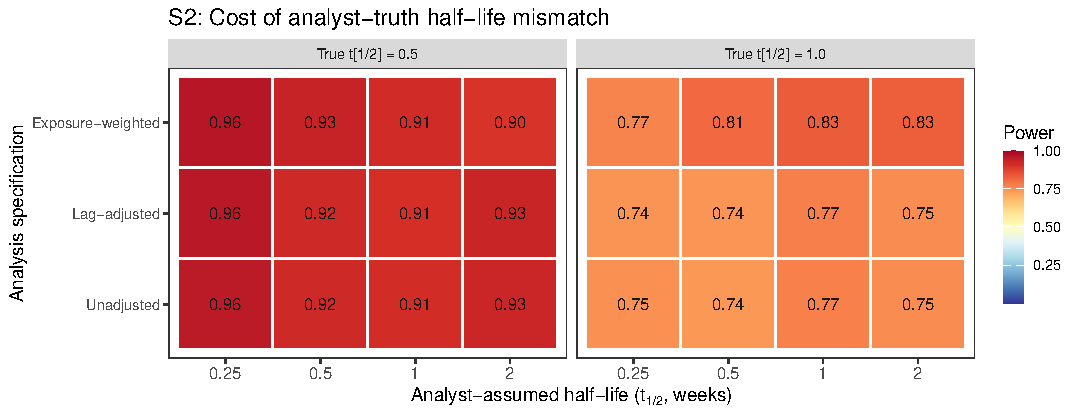
\includegraphics[width=0.9\linewidth]{../../figures/02xs-heatmap-sens-S2} \caption{Block S2: power by analyst-assumed half-life and analysis specification, faceted by true half-life, same data as the line plot above.}\label{fig:fig-heatmap-sens-s2}
\end{figure}

\begin{figure}
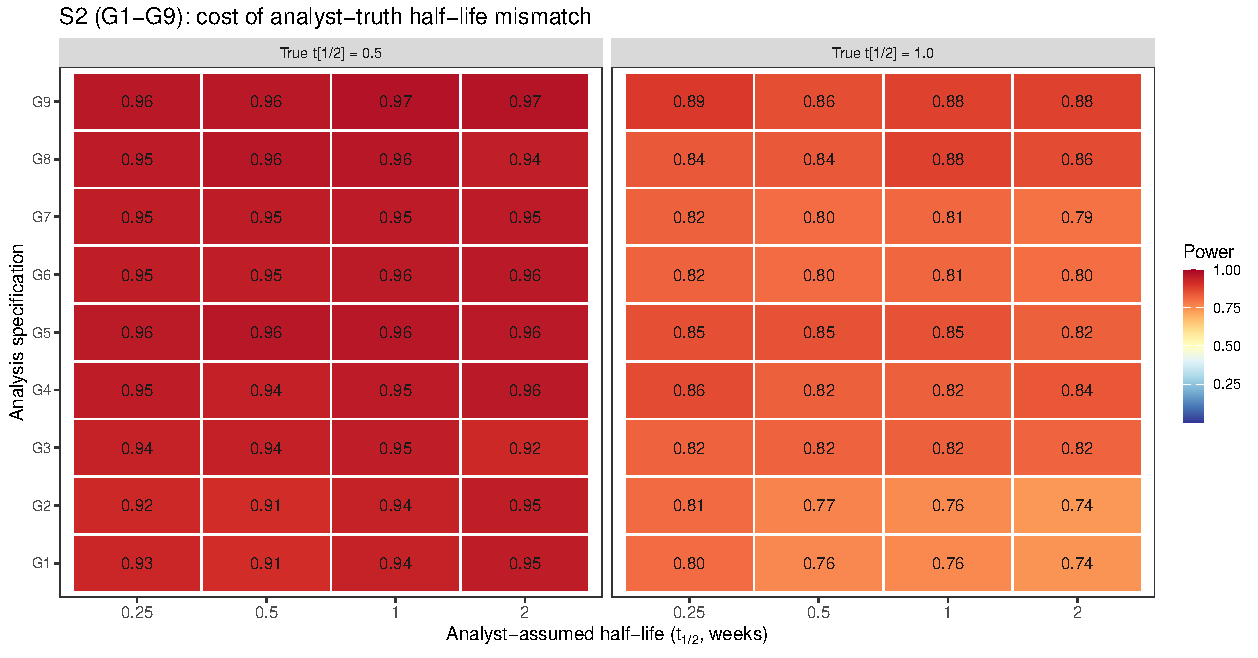
\includegraphics[width=0.95\linewidth]{../../figures/02xs-heatmap-sens-S2-g9} \caption{Block S2 extended to all nine G1-G9 specifications (preliminary $n_{sim} = 100$).}\label{fig:fig-heatmap-sens-s2-g9}
\end{figure}

Block S2 crosses two true half-lives (\(t_{1/2} \in \{0.5, 1.0\}\)
weeks) with four analyst-assumed values (\(\hat{t}_{1/2} \in \{0.25,
0.5, 1.0, 2.0\}\) weeks), giving eight cells. Only Exposure-weighted
consumes \(\hat{t}_{1/2}\), so the cost of a wrong assumption must be
read within a true half-life rather than pooled across the block.

The penalty is modest. At a true half-life of 1.0 weeks,
Exposure-weighted attains 0.832 correctly specified, versus 0.766,
0.808, and 0.826 at assumed values of 0.25, 0.5, and 2.0 weeks. The
worst case, a fourfold under-assumption, costs 6.6 points and still
leaves it above both alternatives (0.746, 0.742). At a true
half-life of 0.5 weeks it attains 0.934 correctly specified, against
0.964, 0.914, and 0.896 at the same four assumed values. Because
Unadjusted and Lag-adjusted cannot depend on \(\hat{t}_{1/2}\), their
variation along that axis is pure Monte Carlo error, ranging 0.910
to 0.960 at a true half-life of 0.5 weeks. This roughly four- to
five-point noise floor explains the apparent anomaly that assuming
0.25 weeks (0.964) beats correct specification (0.934), a difference
well inside it. It also qualifies the one case where the direction
is worth noting. At a true half-life of 0.5 weeks with an assumed
value of 2.0 weeks, Exposure-weighted falls to 0.896, below both
alternatives (0.926, 0.930), so a fourfold over-assumption erodes
its advantage to a tie.

The practical reading, given in the main text, follows from the
limiting-case relationship of Section 2.4: shrinking \(\hat{t}_{1/2}\)
drives the predictor toward the binary indicator, which remains
serviceable, whereas inflating it drives the predictor toward a
constant, at which the on-off contrast and the estimand itself
degenerate.

\section{S4: biomarker-moderation effect-size curve}\label{s4-biomarker-moderation-effect-size-curve}

\begin{figure}
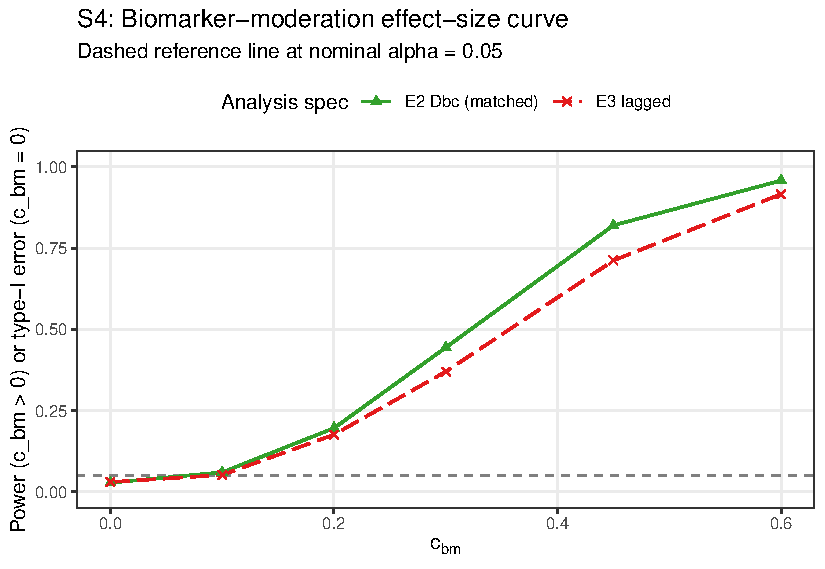
\includegraphics[width=0.6\linewidth]{../../figures/02xs-sens-S4} \caption{Power across the biomarker-moderation effect-size range $c_{bm} \in \{0, 0.10, 0.20, 0.30, 0.45, 0.60\}$. The $c_{bm} = 0$ point is the null for Type I verification.}\label{fig:fig-sens-s4}
\end{figure}

\begin{figure}
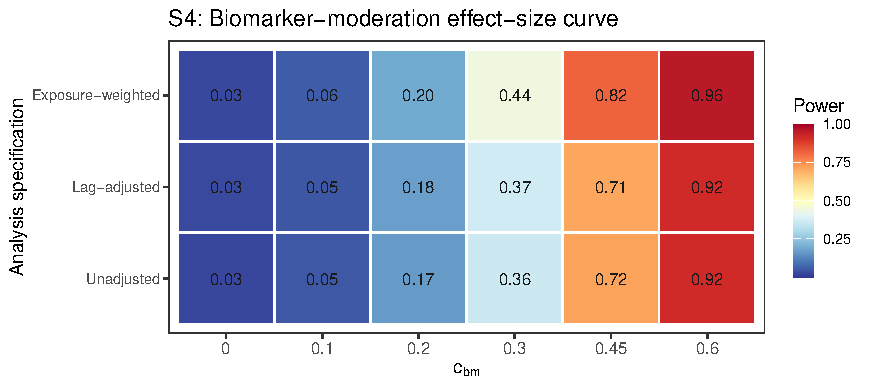
\includegraphics[width=0.7\linewidth]{../../figures/02xs-heatmap-sens-S4} \caption{Block S4: power by biomarker-moderation effect size and analysis specification, same data as the line plot above.}\label{fig:fig-heatmap-sens-s4}
\end{figure}

\begin{figure}
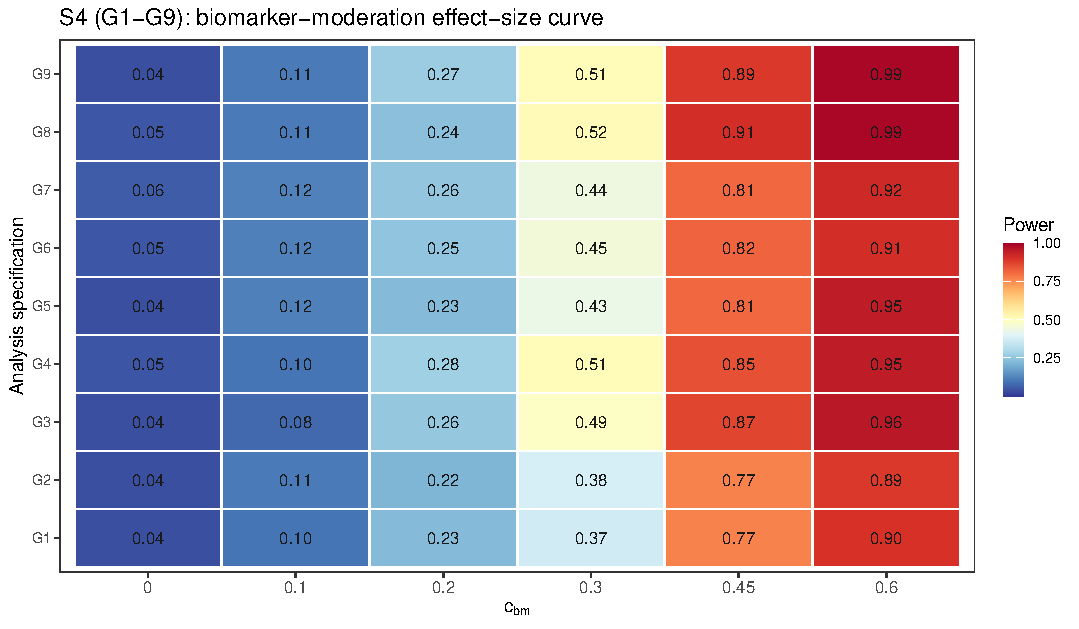
\includegraphics[width=0.8\linewidth]{../../figures/02xs-heatmap-sens-S4-g9} \caption{Block S4 extended to all nine G1-G9 specifications (preliminary $n_{sim} = 100$).}\label{fig:fig-heatmap-sens-s4-g9}
\end{figure}

The power curve is sigmoidal for all three specifications. At
\(c_{bm} = 0\), empirical Type I error sits below nominal for each
(0.026 to 0.030). Power then rises through the mid-range and
saturates once \(c_{bm} \geq 0.45\), reaching 0.916 to 0.958 at
\(c_{bm} = 0.6\). The Exposure-weighted advantage over the unadjusted
benchmark is largest at intermediate effect sizes, \(+0.082\) absolute
at \(c_{bm} = 0.30\) and \(+0.102\) at \(c_{bm} = 0.45\), shrinking to
\(+0.042\) at \(c_{bm} = 0.60\) as all three approach the ceiling, so
the advantage matters most for trials targeting a moderate
biomarker-treatment interaction. Lag-adjusted and Unadjusted
coincide across the entire range, differing by at most 0.008.

\section{S8: architecture sensitivity, full detail}\label{s8-architecture-sensitivity-full-detail}

The main text (Section 3.6) reports this block's headline finding:
\texttt{E7} and \texttt{E9} both beating the unadjusted benchmark at the Hybrid
reference cell is architecture-specific, joining Exposure-weighted
in a pattern that grows with carryover severity, and Lag-adjusted
remains indistinguishable from Unadjusted under both architectures.
Full cell-by-cell detail follows.

Every result reported in the main text, Tier 1 and blocks S1-S7
alike, is restricted to Architecture B (covariance moderation), the
manuscript's stated scope (Section 2.3). Block S8 asks a narrower
question than a full architecture comparison, which is the purpose
of the companion manuscript on DGP architectures\textsuperscript{\citeproc{ref-pmsimstats_dgp_architectures2026}{1}}: does the ranking among analysis
specifications established under Architecture B hold under
Architecture A (mean moderation) as well, or is the choice of
carryover representation itself architecture-dependent? We refit the
five specifications of block S7's table (\texttt{E1}, Lag-adjusted \texttt{E3},
Exposure-weighted \texttt{E2}, \texttt{E7}, \texttt{E9}) at the same reference cell under
both architectures, at three half-lives (\(t_{1/2} \in \{0, 0.5,
1.0\}\)) rather than the single reference value, so the check covers
whether the ranking is architecture-dependent uniformly or only once
carryover is severe enough. Because \(c_{bm}\) is not calibrated to
equal power across architectures, the two produce materially
different absolute power at the same nominal value (Section 1;\textsuperscript{\citeproc{ref-pmsimstats_dgp_architectures2026}{1}} shows the mean-moderation channel
requires several times the nominal effect size for a comparable
power loss under carryover); only the within-architecture ranking is
the object of interest here.

\begin{table}
\centering
\caption{\label{tab:tab-s8}Block S8: analysis-specification ranking by DGP
    architecture and carryover half-life, at the reference cell
    (Hybrid, $N = 70$, $c_{bm} = 0.45$, exponential DGP,
    $n_{sim} = 500$). Absolute power is not comparable between
    architectures at the same nominal $c_{bm}$; only the
    within-architecture ranking is of interest.}
\centering
\resizebox{\ifdim\width>\linewidth\linewidth\else\width\fi}{!}{
\fontsize{9}{11}\selectfont
\begin{tabular}[t]{lrlll}
\toprule
Architecture & t1/2 & Specification & Power (MCSE) & Non-conv\\
\midrule
B (covariance) & 0.0 & Unadjusted & 0.982 (0.006) & 0.000\\
B (covariance) & 0.0 & Lag-adjusted & 0.980 (0.006) & 0.000\\
B (covariance) & 0.0 & Exposure-weighted & 0.982 (0.006) & 0.000\\
B (covariance) & 0.0 & AIC-selected t1/2 & 0.980 (0.006) & 0.000\\
B (covariance) & 0.0 & Paired-difference & 0.974 (0.007) & 0.000\\
\addlinespace
B (covariance) & 0.5 & Unadjusted & 0.922 (0.012) & 0.000\\
B (covariance) & 0.5 & Lag-adjusted & 0.920 (0.012) & 0.000\\
B (covariance) & 0.5 & Exposure-weighted & 0.936 (0.011) & 0.000\\
B (covariance) & 0.5 & AIC-selected t1/2 & 0.936 (0.011) & 0.002\\
B (covariance) & 0.5 & Paired-difference & 0.934 (0.011) & 0.000\\
\addlinespace
B (covariance) & 1.0 & Unadjusted & 0.760 (0.019) & 0.000\\
B (covariance) & 1.0 & Lag-adjusted & 0.760 (0.019) & 0.000\\
B (covariance) & 1.0 & Exposure-weighted & 0.836 (0.017) & 0.000\\
B (covariance) & 1.0 & AIC-selected t1/2 & 0.850 (0.016) & 0.000\\
B (covariance) & 1.0 & Paired-difference & 0.842 (0.016) & 0.000\\
\addlinespace
A (mean) & 0.0 & Unadjusted & 0.972 (0.007) & 0.000\\
A (mean) & 0.0 & Lag-adjusted & 0.972 (0.007) & 0.000\\
A (mean) & 0.0 & Exposure-weighted & 0.972 (0.007) & 0.000\\
A (mean) & 0.0 & AIC-selected t1/2 & 0.970 (0.008) & 0.000\\
A (mean) & 0.0 & Paired-difference & 0.942 (0.010) & 0.000\\
\addlinespace
A (mean) & 0.5 & Unadjusted & 0.968 (0.008) & 0.000\\
A (mean) & 0.5 & Lag-adjusted & 0.968 (0.008) & 0.000\\
A (mean) & 0.5 & Exposure-weighted & 0.966 (0.008) & 0.000\\
A (mean) & 0.5 & AIC-selected t1/2 & 0.970 (0.008) & 0.002\\
A (mean) & 0.5 & Paired-difference & 0.960 (0.009) & 0.000\\
\addlinespace
A (mean) & 1.0 & Unadjusted & 0.972 (0.007) & 0.000\\
A (mean) & 1.0 & Lag-adjusted & 0.976 (0.007) & 0.000\\
A (mean) & 1.0 & Exposure-weighted & 0.946 (0.010) & 0.000\\
A (mean) & 1.0 & AIC-selected t1/2 & 0.950 (0.010) & 0.000\\
A (mean) & 1.0 & Paired-difference & 0.964 (0.008) & 0.000\\
\bottomrule
\end{tabular}}
\end{table}

\begin{figure}
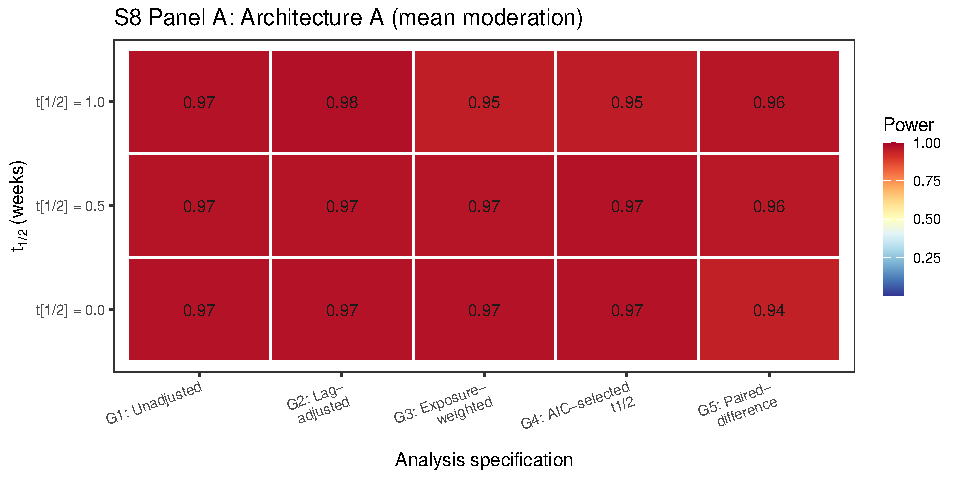
\includegraphics[width=0.8\linewidth]{../../figures/02xs-heatmap-sens-S8-a} \caption{Block S8, Panel A (Architecture A, mean moderation): power by carryover half-life (rows) and analysis specification (columns). Same data as the Architecture A rows of the table above.}\label{fig:fig-heatmap-sens-s8a}
\end{figure}

\begin{figure}
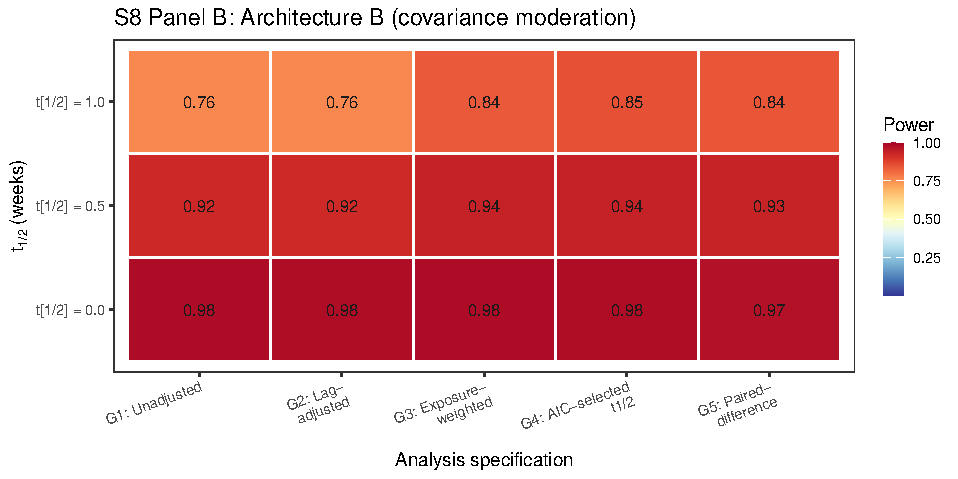
\includegraphics[width=0.8\linewidth]{../../figures/02xs-heatmap-sens-S8-b} \caption{Block S8, Panel B (Architecture B, covariance moderation): power by carryover half-life (rows) and analysis specification (columns). Same data as the Architecture B rows of the table above. Not directly comparable to Panel A in absolute terms.}\label{fig:fig-heatmap-sens-s8b}
\end{figure}

Table \ref{tab:tab-s8} and Figures \ref{fig:fig-heatmap-sens-s8a}/
\ref{fig:fig-heatmap-sens-s8b} show the S7 result (\texttt{E7} and \texttt{E9}
both beating \texttt{E1}) is architecture-specific, joining Exposure-weighted
in a pattern that grows with carryover severity rather than
switching on at some threshold. At \(t_{1/2} = 0\) every specification
collapses to nearly the same value in both architectures (no
carryover to represent), so \texttt{E1}, \texttt{E2}, and \texttt{E7} agree there by
construction (all \(0.97\)-\(0.98\) under B, \(0.97\) under A); \texttt{E9}'s
slightly lower value even at \(t_{1/2} = 0\) (\(0.974\) under B, \(0.942\)
under A) reflects sampling variance in its two-stage estimator
rather than a carryover effect. Under Architecture B, the ranking at
\(t_{1/2} = 1.0\) is \texttt{E7} (\(0.850\)) \textgreater{} \texttt{E9} (\(0.842\)) \textgreater{} \texttt{E2} (\(0.836\)) \textgreater{}
\texttt{E1}/\texttt{E3} (\(0.760\)): both new specifications not only beat the
unadjusted benchmark, as in block S7, but slightly exceed
Exposure-weighted, the manuscript's own current recommendation. At
\(t_{1/2} = 0.5\) the same ordering holds but compressed (\texttt{E7} \(0.936\)
essentially ties \texttt{E2} \(0.936\); \texttt{E9} \(0.934\) close behind; \texttt{E1}/\texttt{E3}
\(0.920\)-\(0.922\) trail by about 1.5 points). Under Architecture A the
pattern reverses for \texttt{E7} and \texttt{E2} alike. At \(t_{1/2} = 1.0\),
\texttt{E1}/\texttt{E3} lead (\(0.972\)/\(0.976\)), \texttt{E9} trails only slightly (\(0.964\),
a \(0.8\)-point gap), while \texttt{E2} (\(0.946\)) and \texttt{E7} (\(0.950\)) trail
more substantially (about 2.2 to 2.6 points, roughly 1.5 MCSE and so
a real, if modest, reversal rather than pure noise). This matches
the pattern already reported from the full-scope grid in the
archived drafts, that Exposure-weighted is marginally dominated in
every design examined under mean moderation (Section 4.6 of the main
text); \texttt{E7} inherits that same architecture-sensitivity since it is
built on Exposure-weighted's formula. \texttt{E9}, built on nothing but a raw
on-drug/off-drug contrast, is comparatively more robust to
architecture, small under B, smaller still under A, though never
reversing to a large disadvantage either way. Lag-adjusted (\texttt{E3})
remains statistically indistinguishable from Unadjusted (\texttt{E1}) under
both architectures at every half-life (largest gap \(0.004\), well
under one MCSE), extending Section 3.3's clean null to Architecture A
as well. The one specification recommendation the main manuscript
makes, exposure weighting in the Hybrid and OL+BDC designs
(Conclusions), is therefore itself conditional on Architecture B and
grows more important as carryover worsens; the same qualification
now extends to \texttt{E7}. \texttt{E9} is the one specification in this table
whose advantage, where it exists, does not appear to depend on which
architecture generated the data, though it was tested only at this
one design and reference cell.

\section{S10: does a CR2 correction change the ranking among G1-G9?}\label{s10-does-a-cr2-correction-change-the-ranking-among-g1-g9}

The main text (Section 3.6) reports this block's headline finding:
CR2 helps every specification it was applied to, and lifts \texttt{G4}
enough that \texttt{G9} (\texttt{G4}+CR2) overtakes every other specification
tested. Full detail follows.

Section 3.5 (Block S6) showed the model-based interaction test is
mildly conservative and that a CR2 cluster-robust standard error
recovers two to five points of power without disturbing the ranking
among \texttt{E1}, \texttt{E2}, and \texttt{E3}. That correction had not been applied to
\texttt{E7} or \texttt{E9}. This block asks two questions at once, adding a compact
naming layer (\texttt{G1}-\texttt{G9}) for the resulting nine-way comparison: does
CR2 help \texttt{E7} and \texttt{E1}/\texttt{E3} the way it already helps \texttt{E2}
(Section 3.5), and does it change which specification leads at the
Hybrid, Architecture B reference cell? \texttt{G1}-\texttt{G5} are the five
specifications introduced so far (\texttt{E1}, \texttt{E3}, \texttt{E2}, \texttt{E7}, \texttt{E9},
respectively); \texttt{G6}-\texttt{G9} cross the CR2 correction with \texttt{G1}, \texttt{G2},
\texttt{G4}, and \texttt{G3}. \texttt{G8} (\texttt{E2}+CR2) already exists as Block S6's
reference-cell result and is included here from that independent run
(different seed, not sharing common random numbers with \texttt{G1}-\texttt{G7}/\texttt{G9},
so its comparison to the rest of this panel is not as tightly paired
as the comparisons among \texttt{G1}-\texttt{G7}/\texttt{G9} are with each other). A tenth
combination, \texttt{G5}+CR2, is not included: \texttt{E9}'s paired-difference
regression collapses to one row per patient before fitting, so there
is no repeated-measures cluster structure left for CR2 to correct.

\begin{table}
\centering
\caption{\label{tab:tab-s10}Block S10: G1-G9 at the reference cell (Hybrid, $N = 70$,
    $c_{bm} = 0.45$, $t_{1/2} = 1.0$, exponential DGP, Architecture B,
    $n_{sim} = 500$). G1-G7 and G9 share common random numbers within
    this block; G8 is from the independent Block S6 run (different
    seed) and is not paired with the rest.}
\centering
\resizebox{\ifdim\width>\linewidth\linewidth\else\width\fi}{!}{
\begin{tabular}[t]{llll}
\toprule
Code & Method & Power (MCSE) & Non-conv\\
\midrule
G1 & Unadjusted & 0.748 (0.019) & 0.000\\
G2 & Lag-adjusted & 0.748 (0.019) & 0.000\\
G3 & Exposure-weighted & 0.826 (0.017) & 0.000\\
G4 & AIC-selected t1/2 & 0.832 (0.017) & 0.000\\
G5 & Paired-difference & 0.804 (0.018) & 0.000\\
\addlinespace
G6 & Unadjusted + CR2 & 0.776 (0.019) & 0.010\\
G7 & Lag-adjusted + CR2 & 0.764 (0.019) & 0.016\\
G8 & Exposure-weighted + CR2 & 0.863 (source: Block S6) & --\\
G9 & AIC-selected t1/2 + CR2 & 0.870 (0.015) & 0.000\\
\bottomrule
\end{tabular}}
\end{table}

\begin{figure}
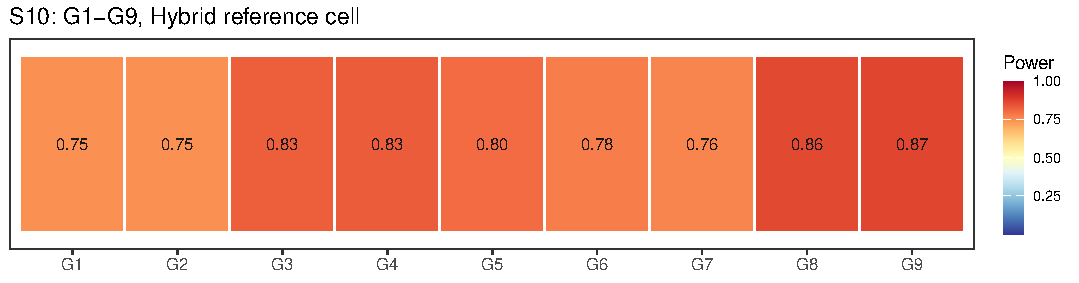
\includegraphics[width=0.95\linewidth]{../../figures/02xs-heatmap-sens-S10} \caption{Block S10: power for G1 through G9 at the Hybrid, Architecture B reference cell, same figures as the table above.}\label{fig:fig-heatmap-sens-s10}
\end{figure}

Table \ref{tab:tab-s10} and Figure \ref{fig:fig-heatmap-sens-s10}
answer both questions together. CR2 helps every specification it was
applied to, consistent with Section 3.5: \texttt{G1}/\texttt{G2} (Unadjusted and
Lag-adjusted, both \(0.748\) model-based) rise to \texttt{G6} \(0.776\) and \texttt{G7}
\(0.764\), gains of \(2.8\) and \(1.6\) points respectively, in line with
the two to five points Block S6 already documented for \texttt{E2}. The
ranking among the five base specifications is unchanged by these
particular gains, since \texttt{G1}/\texttt{G2} remain well below \texttt{G3}-\texttt{G5}
regardless. What does change the ranking is \texttt{G9}. CR2 lifts \texttt{G4}
(AIC-selected half-life, \(0.832\) model-based) to \(0.870\), a \(3.8\)-point
gain, larger than any other CR2 correction observed here or in Block
S6, and enough for \texttt{G9} to overtake every other specification tested,
including \texttt{G8} (\(0.863\), the Block S6 reference-cell result for
Exposure-weighted+CR2). \texttt{G9}'s gain is also notable for what did not
happen: \texttt{E7}'s AIC-selection step raised a Type I error concern
earlier in this manuscript's development (post-selection inference,
since the same data are used to choose the half-life and then test
the resulting coefficient), and one might have expected a CR2
correction, which widens standard errors, to partly offset an
anti-conservative test by coincidence. Instead every replicate
converged under \texttt{G9} (zero non-convergence, against \(1.0\%\) and
\(1.6\%\) for \texttt{G6}/\texttt{G7}), and the power gain is the largest observed,
which is at least consistent with (though does not itself establish)
CR2 correcting real conservatism rather than papering over a
different problem. This block did not test the null (\(c_{bm} = 0\)),
so it does not resolve whether \texttt{G4}/\texttt{G9}'s Type I error is controlled;
Section S11, next, checks that directly.

\section{S11: is G4's Type I error controlled?}\label{s11-is-g4s-type-i-error-controlled}

\texttt{G4} selects its half-life by AIC and then tests the interaction
coefficient from the selected model, a post-selection inference
problem: the same data drive both the selection and the test, which
can in principle inflate Type I error beyond nominal. This had not
been checked anywhere in this manuscript's development. Block S11
tests it directly, refitting \texttt{G1}-\texttt{G5} and \texttt{G9} at the null
(\(c_{bm} = 0\)) at the Hybrid reference cell, with \(n_{sim} = 2000\)
for tighter precision on a rate expected near \(0.05\).

\begin{figure}
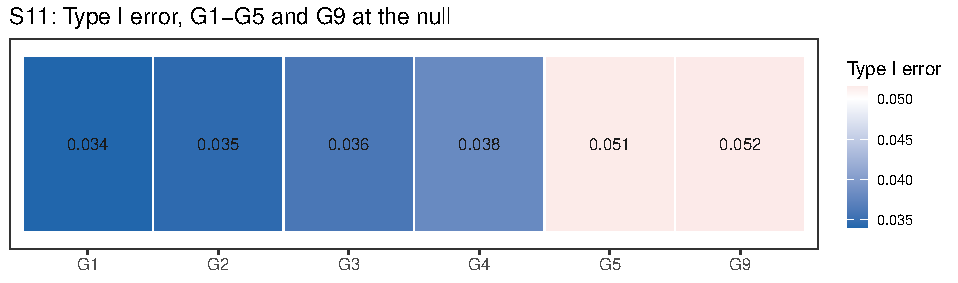
\includegraphics[width=0.8\linewidth]{../../figures/02xs-heatmap-sens-S11} \caption{Block S11: empirical Type I error under the null for G1-G5 and G9 (diverging scale centered at nominal 0.05).}\label{fig:fig-heatmap-sens-s11}
\end{figure}

The concern does not materialize. \texttt{G4}'s Type I error is \(0.038\)
(MCSE \(0.004\)), conservative and in the same range as \texttt{G1}-\texttt{G3}
(\(0.034\)-\(0.036\)), not inflated by the selection step; if anything it
sits slightly closer to nominal than \texttt{G1}/\texttt{G3}. \texttt{G9} (\texttt{G4}+CR2) is
\(0.052\), indistinguishable from nominal \(0.05\) (well under one MCSE),
matching \texttt{G5}'s own \(0.052\). Non-convergence for \texttt{G4}/\texttt{G9} was
negligible (\(0.05\%\), one replicate of 2000). Read together with
Section S10's power results, this means \texttt{G9}'s status as the
best-performing specification in Section S10 is not an artifact of an
uncontrolled test: it wins on power while holding Type I error at
nominal, the same standard \texttt{G3}+CR2 (\texttt{G8}) is held to. This does not
generalize beyond the single cell tested; the post-selection
inference risk that motivated this block is a property of the
estimator, not of this specific cell, but only this cell was checked.

\section{S12: Architecture A counterpart to Figures 1-3 (exploratory)}\label{s12-architecture-a-counterpart-to-figures-1-3-exploratory}

The main manuscript restricts every result except Block S8 to
Architecture B (covariance moderation), the scope stated in Section
2.3. This section is exploratory material outside that scope: an
Architecture A (mean moderation) counterpart to the main
manuscript's Figures 1-3, generated on request for comparison. It is
not part of this manuscript's evidence base and is not referenced by
any claim in the main text.

Panels A and B (all nine specifications) are from a dedicated 30-cell
simulation restricted to Architecture A, otherwise identical in
design to the Architecture B simulation behind the main manuscript's
Figures 1-2 (\texttt{21-run-tier1-hendrickson-g9-archA.R}, \(n_{sim} = 250\),
after a 100-rep smoke test passed sanity checks: no missing values,
power spanning 0.02-0.98, mean non-convergence 0.08\%, no cell above
2\%). Panel C (\texttt{G1}-\texttt{G3} only, decay-shape axis) needs no new
simulation: the production Tier 1 grid already crosses both
architectures at \(n_{sim} = 500\), so this panel is read directly from
existing data at full production precision, unlike Panels A and B.

\begin{figure}
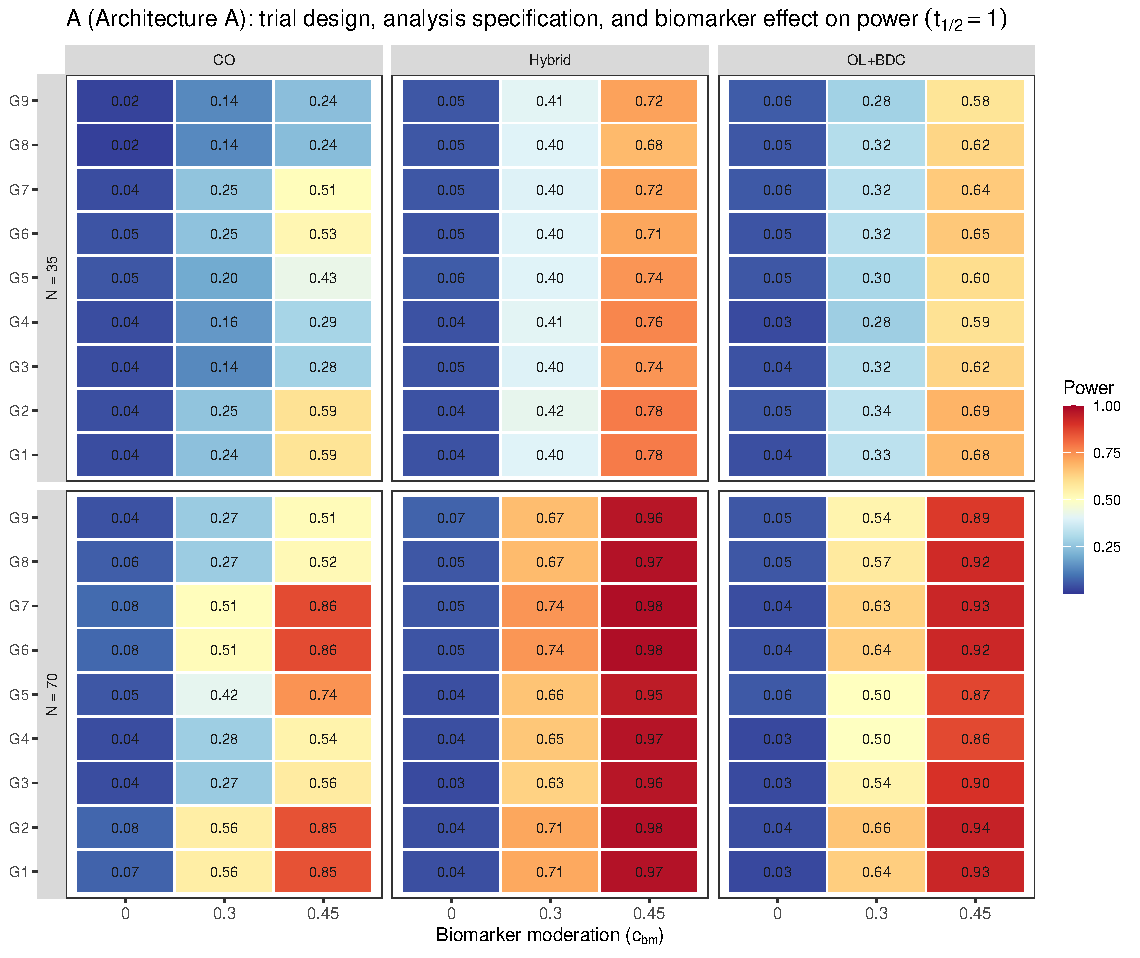
\includegraphics[width=0.95\linewidth]{../../figures/02xs-heatmap-hendrickson-a-archA} \caption{Architecture A counterpart to Figure 1: biomarker-effect axis, all nine G1-G9 specifications, power by trial design (columns), $N$ (row blocks), and analysis specification (rows within block), across $c_{bm} \in \{0, 0.30, 0.45\}$ at $t_{1/2} = 1.0$ weeks, exponential DGP, Architecture A ($n_{sim} = 250$).}\label{fig:fig-hendrickson-a-archA}
\end{figure}

\begin{figure}
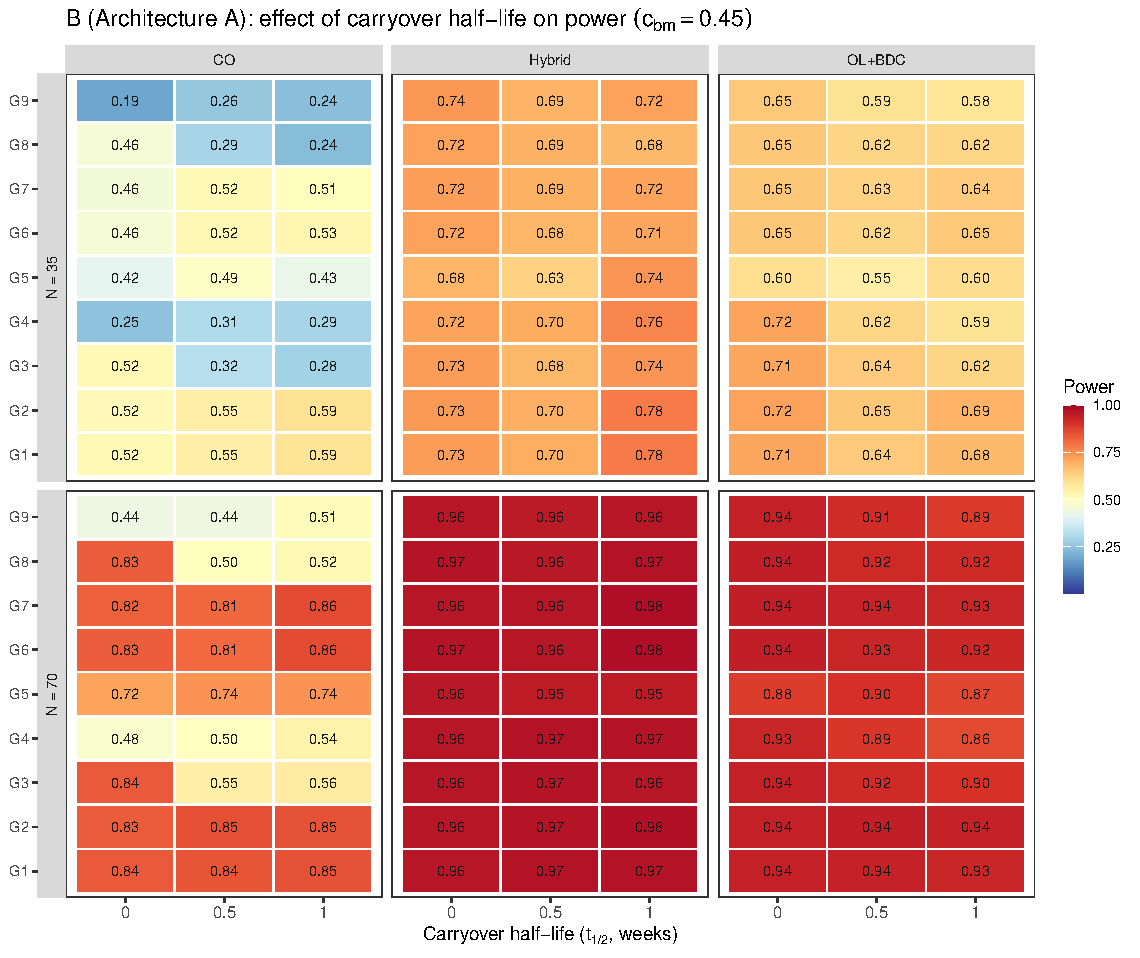
\includegraphics[width=0.95\linewidth]{../../figures/02xs-heatmap-hendrickson-b-archA} \caption{Architecture A counterpart to Figure 2: carryover-axis, all nine G1-G9 specifications, power by trial design (columns), $N$ (row blocks), and analysis specification (rows within block), across $t_{1/2} \in \{0, 0.5, 1.0\}$ weeks at $c_{bm} = 0.45$, exponential DGP, Architecture A ($n_{sim} = 250$).}\label{fig:fig-hendrickson-b-archA}
\end{figure}

\begin{figure}
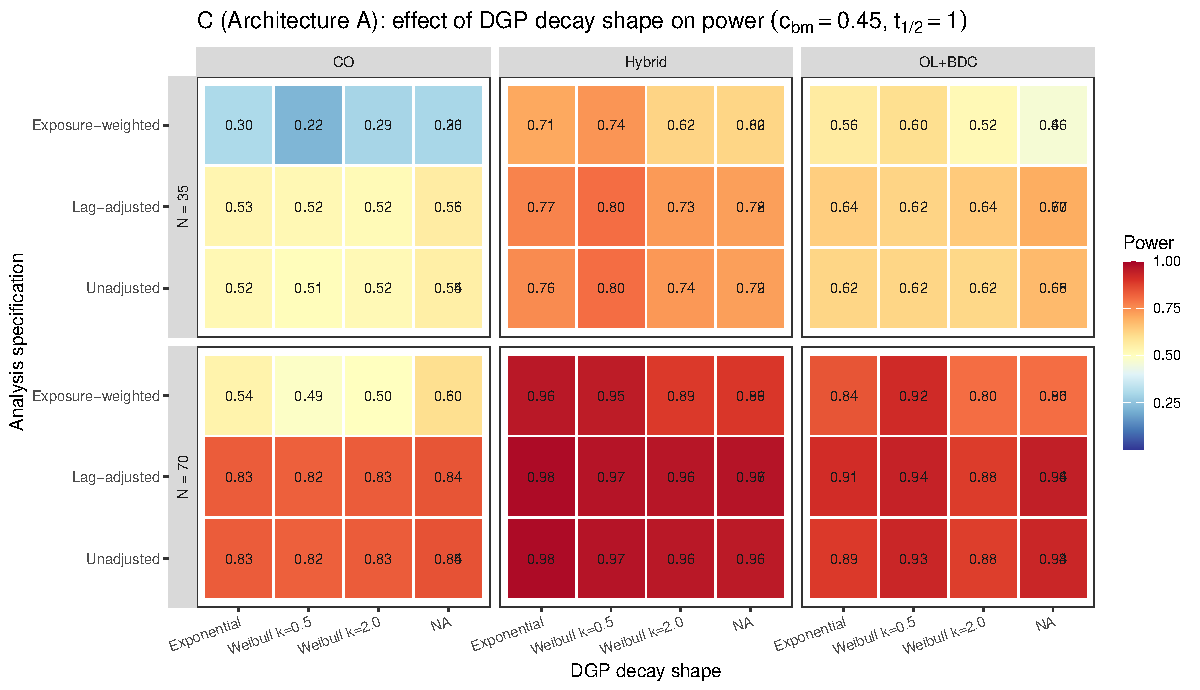
\includegraphics[width=0.95\linewidth]{../../figures/02xs-heatmap-hendrickson-c-archA} \caption{Architecture A counterpart to Figure 3: decay-shape axis, power by trial design (columns), $N$ (row blocks), and analysis specification (rows within block), across the four DGP decay-shape levels (exponential, Weibull $k \in \{0.7, 1.0, 1.5\}$) at $c_{bm} = 0.45$, $t_{1/2} = 1.0$ weeks, Architecture A ($n_{sim} = 500$).}\label{fig:fig-hendrickson-c-archA}
\end{figure}

This is consistent with, and considerably sharper than, Block S8's
finding (Section 3.7 of the main text) that the Exposure-weighted
family's advantage is architecture-sensitive. At the CO cell
(\(N = 70\), \(c_{bm} = 0.45\), \(t_{1/2} = 1.0\)), the Exposure-weighted
family trails \texttt{G1}/\texttt{G2}/\texttt{G6}/\texttt{G7} by a similar margin under both
architectures (\texttt{G4} \(0.54\) against \texttt{G1} \(0.85\) here, against \texttt{G4}
\(0.48\) / \texttt{G1} \(0.86\) under Architecture B at the same cell). At
Hybrid, the separation that favors Exposure-weighted under
Architecture B collapses under Architecture A, but not by reversing:
every specification is near ceiling there (\texttt{G1} \(0.972\), \texttt{G3}
\(0.964\), \texttt{G4} \(0.968\), \texttt{G9} \(0.964\)), a compression that likely
reflects Architecture A's mean-moderation channel producing higher
absolute power at this \(c_{bm}\) in a design with abundant on-drug
information, leaving little room for any specification to separate
from another. At OL+BDC the pattern does reverse, modestly: \texttt{G1}
(\(0.928\)) edges out \texttt{G3}/\texttt{G4}/\texttt{G9} (\(0.900\)/\(0.864\)/\(0.888\)) by
3 to 6 points. Readers should treat this section as a first look,
not a validated comparison: a proper cross-architecture comparison,
including the full factorial grid and the sensitivity battery Block
S8 alone does not cover, is the subject of the companion manuscript
on DGP architectures\textsuperscript{\citeproc{ref-pmsimstats_dgp_architectures2026}{1}} and the
archived full-scope drafts.

\protect\phantomsection\label{refs}
\begin{CSLReferences}{0}{1}
\bibitem[\citeproctext]{ref-pmsimstats_dgp_architectures2026}
\CSLLeftMargin{1. }%
\CSLRightInline{{pmsimstats team}. Two architectures for simulating biomarker-treatment interactions in aggregated {N}-of-1 trials. Published online 2026.}

\end{CSLReferences}

\end{document}
